\section{The Cloud-Edge-Mobile Continuum}\label{sec:continuum}

Together, the computational resources from mobile, edge, and cloud computing have the potential of forming a \textit{continuum} on which new and disruptive types of applications can rely (Fig.~\ref{fig:continuum-overral}). Sometimes referred to as the Cloud-to-Things continuum, it enables the seamless convergence of infrastructure stretching from the cloud datacenter to devices on the network edge (including intermediate devices like ISP gateways, cellular base stations, and private cloud deployments) into a continuum of resources, to be provisioned to multiple tenants for hosting applications. Components of an application are hence able to run in a geo-distributed fashion using the services provided by the distributed infrastructure~\cite{GuptaIfogSim17}. 

\begin{figure}[tbp]
	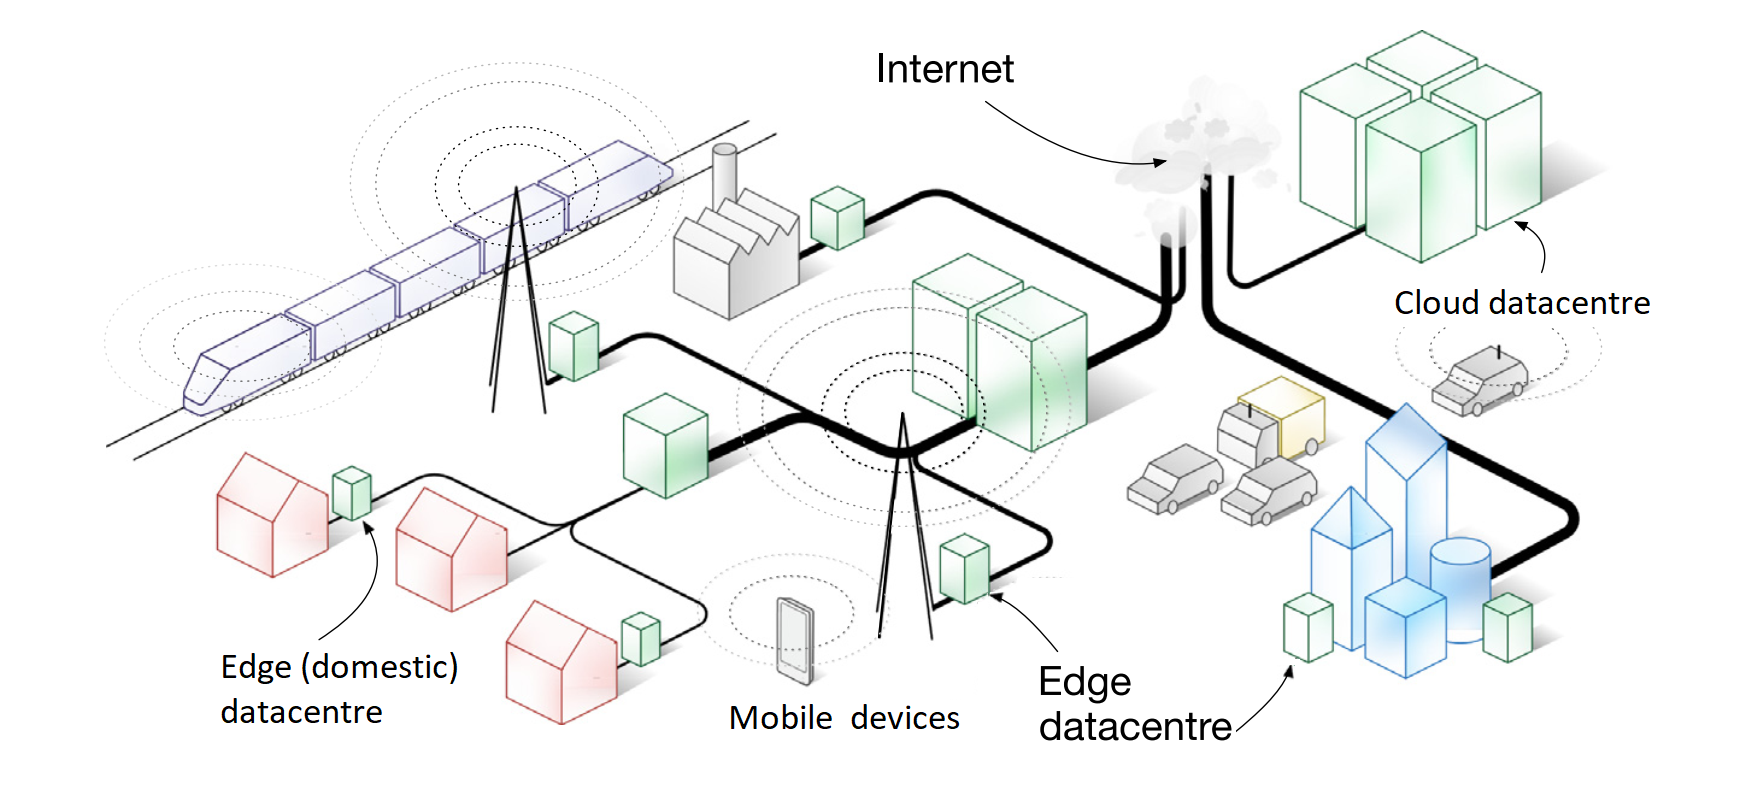
\includegraphics[width=0.9\textwidth]{figs/Continuum-overall.png}
	\caption{The computational continuum formed by coarsely distributed cloud datacenters, finely distributed edge datacenters, and mobile/IoT devices (adapted from~\cite{Tarneberg2017}).}
	\label{fig:continuum-overral}
\end{figure}

The key notion to bridge the gap in such a continuum is that of edge\footnote{In the literature the term ``edge'' is often used interchangeably with the term ``fog''.} computing. The main motivation for shifting computation from cloud to the network edge is the mitigation of network latency~\cite{Bonomi2014}. In specific, real-time applications are the main candidates for benefiting of services deployed at nearby edge infrastructure. For example, Augmented Reality (AR) is a type of application that would benefit from the low-latency of edge services~\cite{GarrigaMendonca2017}. Moreover, despite the significant improvements in the capabilities of mobile devices, the later still suffer from limitations that further motivates the use of edge computing as part of a continuum. In specific, some mobile applications rely on heavyweight tasks that can overstress the platform, imposing battery drain and limiting the concurrent execution of other applications. 


%the battery is a valuable resource that may be significantly affected by the kind of task performed locally, as networking tends to consume less than CPU(s)~\cite{Carroll:2010}. 

%of mobile devices, the later still suffer from battery drain and other platform/hardware limitations which motivates their computation offloading. 
 
%Mobile devices can integrate the continuum as both clients of computation that may opportunistically be offloaded to edge servers and providers of their own local services to cope with the situations in which edge is not available. 


%, whose defining characteristics are edge location, dense geographical distribution, large-scale of deployment, support for mobility, resource and interface heterogeneity, and interplay with the cloud properties in order to address requirements of mobile applications that need low latency with a wide and dense geographical distribution~\cite{Bonomi2014}.  



%\subsection{Cloud Computing}
%
%The Cloud infrastructure is typically offered through different virtualization techniques and degrees~\cite{leitner2016patterns, Quatrocchi2016discrete}. It is considered to be a black box: this means that application developers do not have access to the hypervisor or to the underlying physical machines, which are managed by cloud providers. A Cloud instance or \textit{node} is traditionally materialized as a Virtual Machine (VM). However, nowadays a node might also be a container. Containers provide yet another virtualization technique that operates at the Operating System (OS) level, to create isolated views of the operating environment for different applications. A container has its own process space, virtualized network interface, and file system; and the operating system can allocate different amounts of resources (e.g., CPU, memory, and I/O) to each of them.
%
%Multiple VMs are managed by a single hypervisor that resides on a single host operating system. Each VM then contains its own guest operating system, its own platform stack composed of different libraries, middleware, and application servers, and its own application code. On the other hand, containers are executed directly on top of the host operating system, optionally with the help of a container manager like Docker\footnote{Docker -- \url{http://docker.com}}. Each container has its own platform stack and its own application code. Containers have various advantages when compared to VMs: they are more lightweight and they are faster to boot and terminate because they do not have to deal with a guest
%operating system~\cite{FelterContainerVm15,SoletzContainerVirt14}.
%%Industry is widely adopting containers as a means to favor portability and they are considered to be one of the main technological enablers of the DevOps movement [36]. Different development teams may use different operating systems and different platform stacks, making feature integration hard. However, thanks to containerization technology, features can be developed in isolation, with the guarantee that they will work the exact same way on any machine that supports containers.
%
%\subsection{Edge Computing}
%
%Edge computing can be defined by the set of technologies that enable computation to be performed at the network edge~\cite{Shi:2016}. Its main goal is to allow data produced and consumed at the network edge to be processed with low-latency and without overstressing the more centralized cloud infrastructure.
%
%As examples of edge technologies, Cloudlets~\cite{Satyanarayanan:2009} have been first presented as mobile cloud servers that can be positioned at strategic locations to provide computing resources to resource constrained devices with low-latency. 
%%with expected high density of users (e.g., at concert halls, stadiums) or areas with temporary infrastructure limitations (e.g., after disasters). 
%Additionally, Mobile Edge Computing (MEC)~\cite{ahmed2016isco} relies on cellular infrastructure to enable a low-latency communication between user equipment (i.e., mobile devices) and servers. 
%

%
%\subsection{Mobile}
%
%
%
%\subsection{Definition}

%Fig.~\ref{fig:continuum} describes the different parts of the continuum. Cloud computing features virtually unlimited computational resources and shall remain as the source of services with higher availability. Edge computing, in turn, features low network latency and shall provide services for real-time and delay-sensitive applications. Finally, despite the improvements in the capabilities of mobile devices, the later still suffer from battery drain and other platform/hardware limitations which motivates computation offloading. In addition to the commonly employed mobile-cloud inter-operation, mobile devices can integrate the continuum as both clients of computation that may opportunistically be offloaded to edge servers and providers of their own local services to cope with the situations in which edge is not available. 
%
%\begin{figure}[tbp]
%	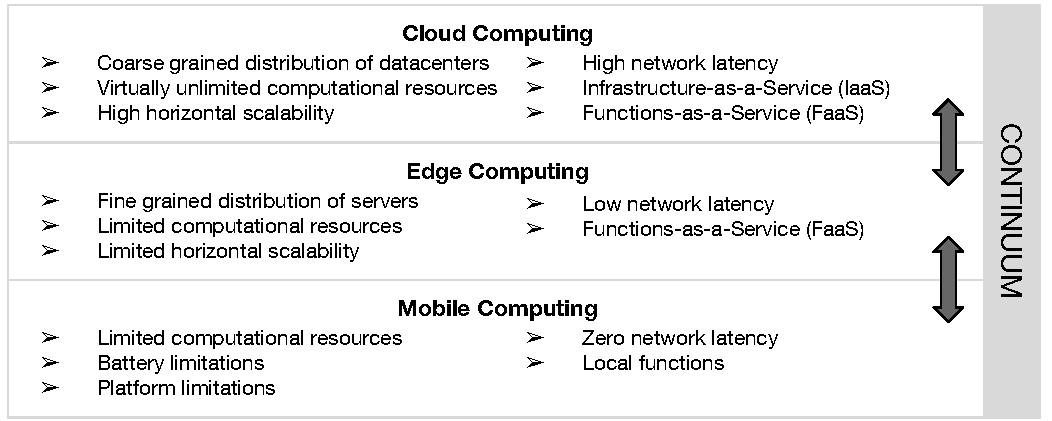
\includegraphics[width=0.9\textwidth]{figs/Continuum.pdf}
%	\caption{Computational continuum formed by Cloud, Edge, and Mobile Computing}
%	\label{fig:continuum}
%\end{figure}

\newcounter{req_count}
\newcounter{req_sub_count}[req_count]


%TODO: parts of this paragraph are unclear (e.g., interplay with the cloud properties?)



%What: the challenges in materializing the continuum
\subsection*{Key Characteristics and Challenges}

%TODO: talk about heterogeneity of cloud, edge, and mobile, not about specific edge details that should be described later
\subsubsection*{Heterogeneity}\label{sec:heterogeneity}

%\stepcounter{req_count}

The continuum encompasses \textit{heterogeneous} types of computing platforms and technologies located at the cloud and at the edge of the network, as well as in mobile devices. Among others, the heterogeneity includes the granularity in which edge datacenters are geographically distributed, posing the challenges of efficiency and scalability; it also includes the way edge services are discovered and accessed, which poses the challenge of awareness. Finally, it includes the particular constraints of mobile devices in terms of battery, platform, and hardware limitations, which adds to the factors that must be taken into account in the decision of where computation should be placed along the continuum in different contexts of operation.

%Next, we identify the key characteristics of the cloud-edge-mobile continuum posing challenges to its realization along with the properties required to address these challenges.

%This heterogeneity poses challenges in terms of how each part of the continuum should allocate its resources to different types of client applications (provisioning) and how these applications should have access to the continuum resources (inter-operation). 

%In particular, 


%The realization of the continuum requires a flexible model that copes with this heterogeneity (Req. \stepcounter{req_sub_count}\textbf{R\arabic{req_count}.\arabic{req_sub_count}}).%, i.e., different instances of the model should address the many particularities in the continuum .
%, i.e., it should be agnostic with respect to the capabilities and specific technology details of different computing platforms and infrastructures in the continuum (Req. \stepcounter{req_sub_count}\textbf{R\arabic{req_count}.\arabic{req_sub_count}}); and 


%\begin{figure}[tbp]
%	\centering
%	\captionsetup[subfigure]{width=0.51\textwidth}	
%	\null\hfill
%	\subfloat[Heterogeneus and independent types of computing platforms and infrastructure (mobile-edge, local-edge, cloud) in range of communication with a mobile device\label{fig:edge-heterogeneity}]{ 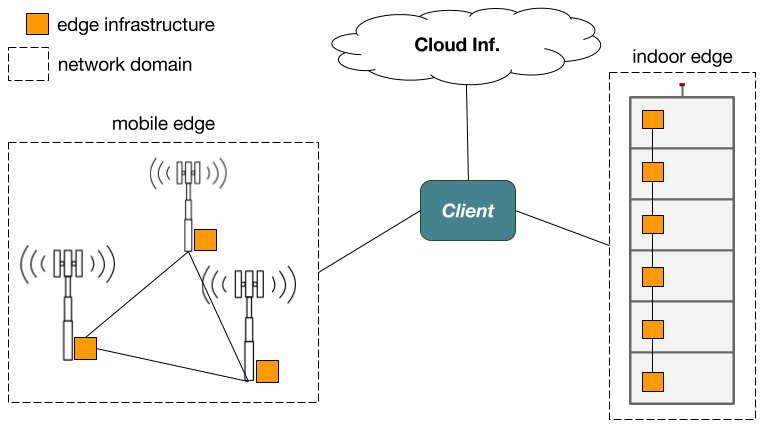
\includegraphics[width=0.51\textwidth]{figs/edge-heterogeneity.png}}
%	\captionsetup[subfigure]{width=0.43\textwidth}	
%	\hfill
%	\subfloat[The heterogeneity of different cloud and edge compute platforms and infrastructures abstracted as domains\label{fig:edge-domain-client}] {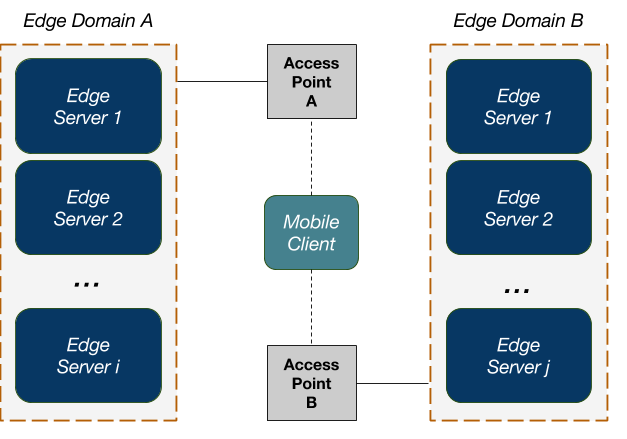
\includegraphics[width=0.43\textwidth]{figs/edge-domain-client.png}}
%	\hfill\null
%	\caption{Continuum heterogeneity}\label{fig:1}
%\end{figure}

%In addition, different kinds of edge infrastructure (e.g., more powerful servers or single board computers) or the same kind of edge infrastructure at different contexts (e.g., the number of clients in an area is too high in one region and low in another) may fit better with different policies for edge resources usage. 

%Client applications heterogeneity
%Client applications may significantly differ in terms of the QoS they require from services and providers. For example, connected vehicles (CV) may eventually rely on edge services for low-latency computation. A CV entering a given region for the first time is unlikely to be waiting until the edge servers covering that region become ready for providing the service the vehicle requires. Conversely, users of an augmented reality application could eventually wait for a setup time whenever the nearby edge \textit{domain}
%%
%~\footnote{From this point on, the term \textit{domain} is used to abstract whatever computational resources can be employed by different computing platforms (i.e., those used by cloud, mobile-edge, local-edge, and local). It is also implied that edge domains are accessible by clients through some (network) access point (Fig.~\ref{fig:edge-domain-client}).} 
%%
%is not ready. 
%%In both cases, low-latency is an important requirement. However, the later type of application could afford a setup delay which the first could not.
%Accordingly, the unified model should enable the co-existence of applications requiring different QoS levels (\stepcounter{req_count}\textbf{R\arabic{req_count}}); and the priority of the usage of computational resources from resource-constrained domains must be in accordance with the application category and its QoS requirements (\stepcounter{req_count}\textbf{R\arabic{req_count}}).

\subsubsection*{Resource Management}\label{sec:efficiency}

\stepcounter{req_count}

In cloud computing, the infrastructure responsible for hosting and performing services is abstracted away from client applications through virtualization and more recently containerization technologies~\cite{leitner2016patterns, Quatrocchi2016discrete}. The horizontal scalability provided by virtually unlimited resources enables elastic services to remain available regardless of the workload.
%by allowing services to remain accessible and operational independently of the number of requests. 
Such a high availability suits well the services covering large or dense areas in which requests are always expected. In contrast, the fine-grained distribution of edge computing suggests that neither computational resources will be abundant, nor the demand for services should be the same as those of cloud-based services. 

%need of a different approach for the provisioning of its resources.  


%The elasticity of cloud datacenters is enabled by its horizontal scalability, in which virtual machines or containers can be instantiated in new virtually unlimited physical resources. 


%...in which backend applications are deployed to virtual machines and/or containers....

%A direct replication of cloud computing IaaS model with edge computing infrastructure would not be possible. 

%First, because it is unlikely that a significant number of applications could be simultaneously hosted by edge servers using technologies such as virtualization and containerization. Even if containers can be allocated faster than virtual machines~\cite{Quatrocchi2016discrete}, at its best, a minimum amount of resources still needs to be allocated to always-deployed containers. Thus, the scalability of edge computing in terms of number of simultaneous services and clients would be reduced. Second, because it is unlikely that clients of services covering small areas shall always be present. 
%To improve efficiency and scalability, the allocation of runtime resources to different services should be opportunistic and without minimum preallocation, unless justified otherwise. % (Req. \stepcounter{req_sub_count}\textbf{R\arabic{req_count}.\arabic{req_sub_count}}). 
%Moreover, the fine-grained distribution of edge computing and its resource limitations also suggests that an a priori installation and deployment to all edge servers would impose unnecessary burden. Even if storage is more abundant and cheaper resource than runtime resources like CPU and memory, a proactive and indiscriminate acquisition of service artifacts could compromise the scalability of edge computing. Instead, the acquisition of service artifacts should be opportunistic, unless justified otherwise. % (Req. \stepcounter{req_sub_count}\textbf{R\arabic{req_count}.\arabic{req_sub_count}}).

\subsubsection*{Locality \& Context-Awareness}\label{sec:context-awareness}

\stepcounter{req_count}

In a fine grained distribution of edge computing, it is unlikely that different service providers will be able to coordinate and decide which one will serve a given client request. For example, from inside a building with some local edge servers accessible through Wi-Fi direct, a client may still be in contact with other servers accessible through 5G\footnote{Fifth generation of broadband cellular technology}. If both providers host the same services, but are unable to communicate and coordinate the allocation of the client request, it is up to the client to make the decision of which provider to use. Accordingly, clients should have the control over which service providers in the continuum should be used. % (Req. \stepcounter{req_sub_count}\textbf{R\arabic{req_count}.\arabic{req_sub_count}}). 

The discovery of finely distributed edge datacenters is another important aspect to be tackled. Today, networking protocols and technologies are the main responsible for allowing client applications to access cloud services in a transparent way. For this, clients access cloud services by means of well-known Internet names that are resolved by traffic managers and domain-name servers (DNS) technologies. The datacenters hosting cloud services are, at best, coarsely distributed among continents, countries, or broader regions. Conversely, finely distributed edge datacenters may be part of the local network infrastructure (e.g., domestic and office infrastructures). Such configuration requires the discovery of local providers by clients. % (Req. \stepcounter{req_sub_count}\textbf{R\arabic{req_count}.\arabic{req_sub_count}}).


%In these cases, services names are mapped to either the servers hosting them or to intermediate components (e.g., traffic managers) responsible for transparently routing client requests to datacenters covering their area. 
%In contrast, in a , a similar transparency may not be possible. 



%Additionally, to allow services to be opportunistically deployed based on the awareness of clients in their coverage area, clients must advertise their requirements to service providers (Req. \stepcounter{req_sub_count}\textbf{R\arabic{req_count}.\arabic{req_sub_count}}).

%clients must be aware of alternative domains (Req. \stepcounter{req_sub_count}\textbf{R\arabic{req_count}.\arabic{req_sub_count}}); and 

%First, because 

%Second, because clients can switch from one network to the other at their discretion or make simultaneous use of different connections.

%Additionally, as mobile clients can enter or exit a given area, their connectivity with a given edge domain may be lost. The less time a mobile client remains connected to a domain, the lower the chances of loosing connection before it is still processing that client's request. Thus, if services are not currently available in one domain, the later should not proxy the request to another domain. Instead, clients should perform direct requests to the cloud instead of having their request forwarded by the edge domain itself.

%In particular, two scenarios of edge computing are possible: 1) edge servers are part of the telecommunications infrastructure (e.g., they are located at cellular base stations); 2) edge servers are part of conventional infrastructure  (e.g., they are located at malls, concert halls, stadiums, office buildings, parks, etc). 
%
%In the first kind of scenario, which correspond to MEC, networking technology could be employed to make the decision of using edge or cloud infrastructure transparent for the client. For instance, active components at the base stations could divert the traffic coming from clients connected to that base station to local edge servers whenever the requested services are available or to the cloud otherwise~\cite{MEC_ROUTING}. 
%
%Analogously, the second kind of scenario would require local network infrastructure components like access points and routers to actively divert the traffic from clients to edge servers in that location upon availability or to the cloud otherwise.
%
%In both cases, clients requests would be transparently handled by either edge or cloud servers, with infrastructure components responsible for taking the edge-or-cloud decision. However, in the event of both types of edge infrastructure to coexist, the client would have to participate of an edge-or-edge kind of decision.


%For instance, at a given moment, the  client device may decide to switch from the mobile-edge domain to the local-edge domain. 

%As such, whereas independent edge servers would not see each other, the client would be able to see them and decide which one suits it the best.

%In addition to the client participation in a edge-or-edge kind of decision, there is an argument in favor of giving the client also the responsibility for the edge-or-cloud type of decision: mobility. 


%\begin{figure}[tbp]
%	\centering
%	\captionsetup[subfigure]{width=0.5\textwidth}	
%	\null\hfill
%	\subfloat[Heterogeneus and indpendent types of edge domains (mobile and indoor) in range of communication with a client device\label{fig:edge-heterogeneity}]{ 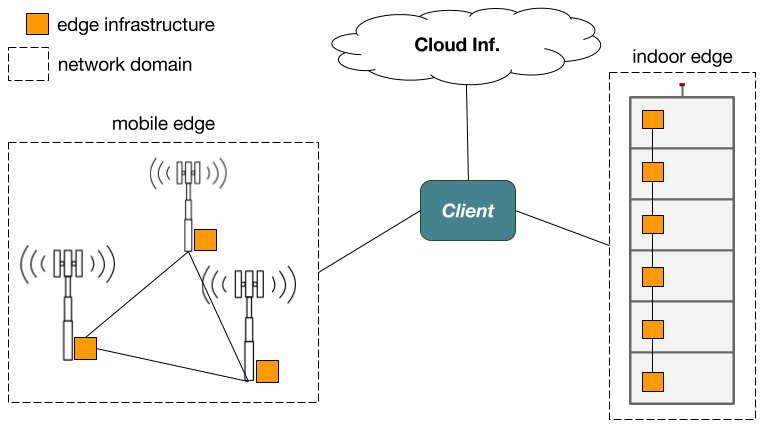
\includegraphics[width=0.5\textwidth]{figs/edge-heterogeneity.png}}
%	\captionsetup[subfigure]{width=0.45\textwidth}	
%	\hfill
%	\subfloat[In the case no edge service is available, client performs direct requests to the cloud and eliminate the dependency with intermediary edge domain infrastructure\label{fig:domain-selection}] {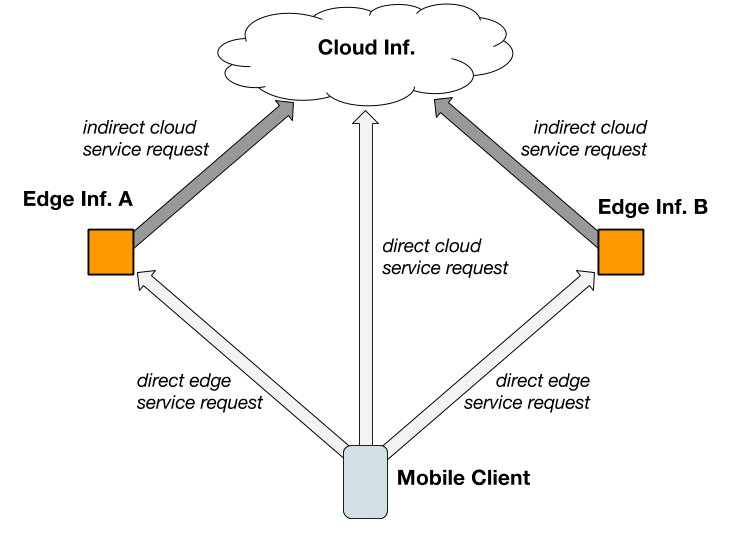
\includegraphics[width=0.45\textwidth]{figs/domain-selection.png}}
%	\hfill\null
%	\caption{Edge heterogeneity and client awareness}\label{fig:no-label-here}
%\end{figure}

%TODO: replace R2 with: Control over forwarding from edge to cloud. Soft vs. strong constraint. Soft = I can also run on cloud if needed. Strong = Never go to cloud.
	
\subsubsection*{Automation and Encapsulation}

\stepcounter{req_count}

Last but not least, the multiplicity of finely distributed edge datacenters implies not only a limitation in terms of availability of resources, but also a large scale of servers to be managed. Such characteristic motivates the automation of the operational aspects of services life-cycle for two reasons: 1) to avoid the burden and costs of manual operation of a large scale of finely distributed servers; and 2) to allow service life-cycle to be efficiently managed. Whereas the later aspect is addressed by the serverless computing paradigm and the FaaS execution model, a complete self-management of services life-cycle is still missing.

%Automation is also needed to allow services to be seamlessly displaced from different parts of the continuum. Accordingly, automation should encompass the operational aspects of services life-cycle, including resource allocation for different services 
%(Req. \stepcounter{req_sub_count}\textbf{R\arabic{req_count}.\arabic{req_sub_count}}) 
%and their installation. 
%(Req. \stepcounter{req_sub_count}\textbf{R\arabic{req_count}.\arabic{req_sub_count}}). 
%Finally, automation should also encompass the choice of alternative services by a client. %(Req. \stepcounter{req_sub_count}\textbf{R\arabic{req_count}.\arabic{req_sub_count}}).


%in the context of a shared platform 

%Following a serverless architecture, the application developer has control over the code they deploy into the infrastructure. 
%The model should be automated and transparent, where the developer is unaware of which infrastructure is using to run her applications. 

%In specific, the allocated resources should be scaled to zero where no servers are actually running when the application's function code is not used, and there is no cost to the user nor overload to the platform.


%Therefore, the management of computational resources must be automated and not depend on  manual intervention from human administrators (\textbf{R\arabic{req_count}}).


%Differently from classical \textit{on-premise} servers, edge should benefit from the automation and other characteristics of the A3-E model. As a result, local-edge servers can be seen as automated black boxes requiring no manual maintenance.	
	
%The fulfillment of the above requirements would leverage the potential of edge computing by optimizing the usage of its resources and consequently allowing a larger number of client applications to share the costs of edge infrastructure. Moreover, the resulting unified model would work as an extension of today's cloud IaaS/FaaS with the twofold purpose of enabling applications with low-latency requirements to rely on edge domains and to augment the computational power of mobile devices through mobile-to-edge computation offloading. Last but not least, the computing power of highly available and elastic cloud services would remain as an essential part of the continuum.

%TODO: talk about what the example applications need; talk about how to solve it later while explaining the proposal
\subsection{Example Scenario}

\begin{figure}[tbp]
	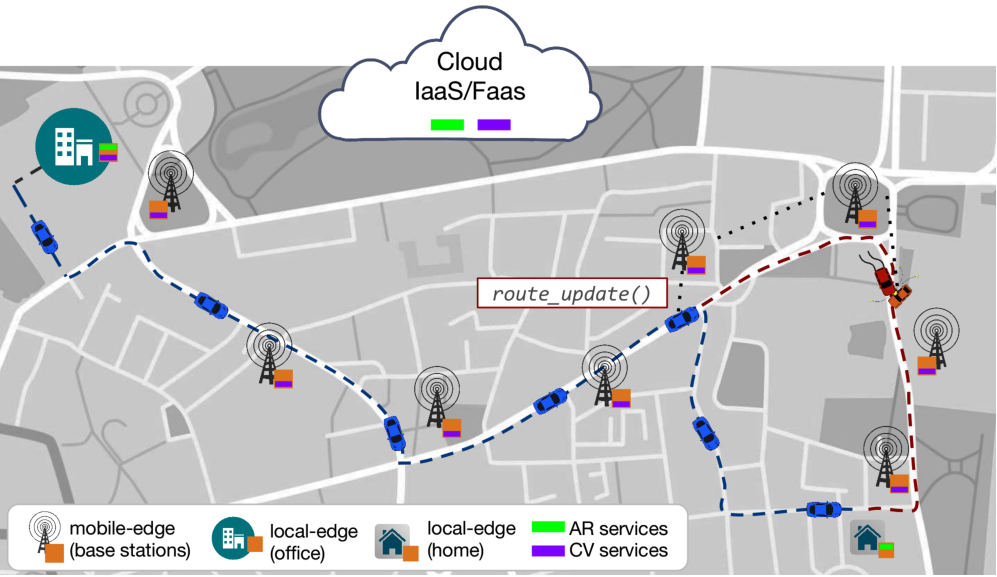
\includegraphics[width=0.8\textwidth]{figs/Continuum-Scenario}
	\caption{Heterogeneous applications such as Augmented Reality (AR) and Autonomous Vehicles (AV) interact with services deployed along the computational continuum (cloud, mobile-edge, local-edge, and mobile)}
	\label{fig:continuum-scenario}
\end{figure}

%Throughout this section an example scenario (Fig.~\ref{fig:continuum-scenario}) is used to illustrate the use of A3-E model and the cloud-edge-mobile continuum with different applications employed by a person with visual impairment.
We illustrate the computational continuum in an example scenario  that starts in a user's office and finishes in his home and involves different applications that rely on services executed in the cloud, edge, or in the user's own devices. 
First, let us assume the existence of a local edge server in the user's office (hereafter called \textit{local-edge}). This server is owned by the company to extend the computational capabilities of devices operated by its employees. In our example, the user makes use of an %Augmented Reality (AR) application that parses objects from scenes captured from his mobile device camera and produces audible information. The application involves two heavyweight tasks: the image processing from the captured scenes ($IP$); and the text-to-speech ($TTS$).
Augmented Reality (AR) application to craft three dimensional virtual objects added to his desk table. In specific, this application involves heavyweight image processing from the captured scenes. By offloading this task to the local-edge, the user is exempt from recharging her glasses and can improve productivity. 

After work, our user leaves his office and enters his Autonomous Vehicle (AV). During its way home, the vehicle will make use of edge services deployed at servers located at cellular base stations (hereafter called \textit{mobile-edge}) to receive low-latency updates about the best plan to reach its destination. Within milliseconds, the vehicle is suggested to make a turn just in time to avoid the traffic formed by an accident a few blocks ahead. In particular, the new path consists of residential streets without coverage of mobile-edge services. The AV continues to fetch updates, this time from cloud services. The additional network latency is compensated with the low speed limit of the residential area.

Already at home, the user's smartphone gets in reach of communication with the local-edge server owned by him. In that day, he finds out about a new mobile game application 
%for visually impaired users
. Upon installation, the edge server becomes aware of a new edge-compliant application and, meanwhile the app is already running locally, proceeds with the setup of required services. Once available, the client application becomes aware of these services and switches from local to edge with the purpose of preserving the smartphone's resources. Not only the game performance improves, but also the battery consumption is reduced.  

In the scenario described above, different parts of the continuum have been employed by user's devices. Whilst edge services were privileged, cloud services remain fundamental, as edge domains were not always available. Furthermore, the edge services consumed by the AR application and those consumed by the AV were pre-allocated by the office's local-edge and the mobile-edge services. In contrast, an AR application was able to make use of local resources from a mobile device until edge services were opportunistically made available by the local-edge server at user's home.

%services for which network latency is not disruptive are in the cloud (e.g., persistence, stateful components, and large part of the business logic).

